\documentclass[10pt]{article}

\usepackage{caption}
\usepackage{subcaption}
\usepackage{subfig}
\usepackage{graphicx}
\usepackage{multirow}
\usepackage{wrapfig}
\usepackage{enumerate}
\usepackage{amsmath}
\usepackage{tabularx}
\usepackage[margin=1.1in]{geometry}

\providecommand{\e}[1]{\ensuremath{\times 10^{#1}}}

\begin{document}

\section{Exercise 1: SVM}

In the general case of solving a linear SVM with slack variables without a regularizer, the objective function is written in Equation \ref{eq:singlesvm} and it's corresponding prediction function and function for calculating $w_0$ in Equation \ref{eq:singlesvm-predictor}.

\begin{subequations}
\begin{align}
	\underset{\alpha}{\text{minimize}}
		& \quad -\sum_{i = 1}^n \alpha_i + \frac{1}{2} \sum_{i = 1}^n \sum_{j = 1}^n \alpha_i \alpha_j y^{(i)} y^{(j)} (x^{(i)} \cdot x^{(j)}) \\
	\text{subject to}
		& \quad 0 \leq \alpha_i \leq C \quad \forall i \,, \\
		& \quad \sum_{i = 1}^n \alpha_i y^{(i)} = 0
\end{align}
\label{eq:singlesvm}
\end{subequations}

\begin{subequations}
\begin{align}
	S & \text{ is the set of support vectors (where )} \alpha > 0 \\
	y(x^{(t)}) &= \text{sign}\left(\sum_{i \in S}^n \alpha_i y^{(i)} (x^{(t)} \cdot x^{(i)}) + w0 \right)\\
	w_0 &= \frac{1}{|S|} \sum_{j \in S} \left(y^{(j)} - \sum_{i \in S} \alpha_i y^{(i)} (x^{(i)} \cdot x^{(j)}) \right)
\end{align}
\label{eq:singlesvm-predictor}
\end{subequations}

Using the Python CVXOPT package, the general form of the objective function is written in Equation \ref{eq:cvxopt}.

\begin{subequations}
\begin{align}
	\underset{x}{\text{minimize}}
		& \quad \frac{1}{2}x^T P x + q^T x \\
	\text{subject to} 
		& \quad Gx \leq h \\
		& Ax = b
\end{align}
\label{eq:cvxopt}
\end{subequations}

The general form for converting our slack variable objective function in Equation \ref{eq:singlesvm} to the CVXOPT objective function in Equation \ref{eq:cvxopt} is described in Table \ref{tbl:cvxopttosvm}.

\begin{table}[!ht]
\centering
\begin{tabular}{c|p{.7\textwidth}}
	CVXOPT& Conversion from Equation \ref{eq:singlesvm} \\ \hline
	$x$ & If there are $n$ points in the training set, an $n \times 1$ vector equal to the values of $x$ in the training data \\
	$P$ & An $n \times n$ matrix which is the kernel matrix between all pairs of training data $x$ weighted by the corresponding value of $y$ from the training data \\
	$q$ & An $n \times 1$ vector of $-1$s \\
	$G$ & A $2n \times n$ matrix where the top $n \times n$ is the identity matrix and the bottom $n \times n$ is the negative identity matrix \\
	$h$ & A $2n \times 1$ vector with the top $n \times 1$ vector of $C$s and the bottom $n \times 1$ vector of $0$s \\
	$A$ & An $1 \times n$ vectors with elements $y^{(i)}$ from the training set for all values of $i$ \\
	$b$ & An $1 \times 1$ vector of $0$s
\end{tabular}
\caption{Conversion rule for deriving CVXOPT constraints}
\label{tbl:cvxopttosvm}
\end{table}

For the small example with $(1,2),(2,2)$ as positive examples and $(0,0),(-2,3)$ as negative examples, the constraints from CVXOPT as written above are written in Equation \ref{eq:1-1}.

\begin{subequations}
\begin{align*}
	P &= \begin{bmatrix}
		5 & 6 & 0 & -4 \\
		6 & 8 & 0 & -2 \\
		0 & 0 & 0 & 0 \\
		-4 & -2 & 0 & 13
	\end{bmatrix} 
	&& q = \begin{bmatrix}
		-1 \\ -1 \\ -1 \\ -1
	\end{bmatrix} \\
	G &= \begin{bmatrix}
		1 & 0 & 0 & 0 \\
		0 & 1 & 0 & 0 \\
		0 & 0 & 1 & 0 \\
		0 & 0 & 0 & 1 \\
		-1 & 0 & 0 & 0 \\
		0 & -1 & 0 & 0 \\
		0 & 0 & -1 & 0 \\
		0 & 0 & 0 & -1
	\end{bmatrix} 
	&& h = \begin{bmatrix}
		1 \\ 1 \\ 1\\ 1\\ 0\\ 0\\ 0\\ 0
	\end{bmatrix}\\
	A &= \begin{bmatrix}
		1 & 1 & -1 & -1	
	\end{bmatrix} 
	&& b = \begin{bmatrix}
		0
	\end{bmatrix}
\end{align*}
\label{eq:1-1}
\end{subequations}

The decision boundary generated by the SVM code for the small example is shown in Figure \ref{fig:1-1}.

\begin{figure}[!ht]
\centering
\begin{subfigure}[b]{0.46\textwidth}
	\centering
	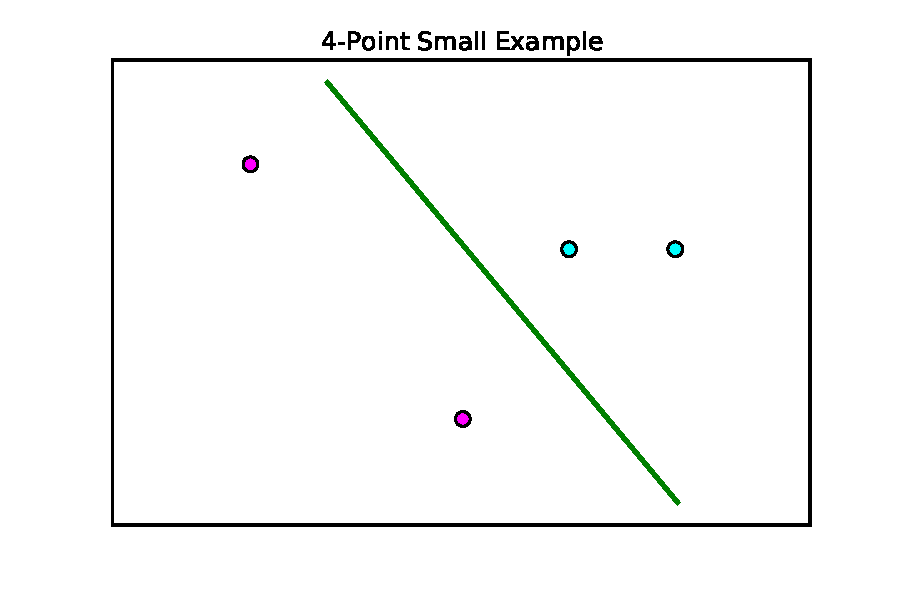
\includegraphics[width=\textwidth]{exercise1-1.pdf}
	\caption{Decision boundary for 4 points using CVXOPT and SVM with slack variables}
	\label{fig:1-1}
\end{subfigure}
\caption{}
\label{fig:1-1-all}
\end{figure}

\begin{table}[!ht]
\centering
\begin{tabular}{r|c|c|c}
	Dataset & Kernel & Training & Validation \\ \hline
	smallOverlap & Linear & $.24$ & $.24$ \\
	smallOverlap & Gaussian $\beta = 0.1$ & $.2$ & $.18$ \\
	smallOverlap & Gaussian $\beta = 1$ & $.05$ & $.05$ \\
	bigOverlap & Linear & $.305$ & $.255$ \\
	bigOverlap & Gaussian $\beta = 0.1$ & $.15$ & $.18$ \\
	bigOverlap & Gaussian $\beta = 1$ & $.1$ & $.08$ \\
	ls & Linear & $0$ & $0.00375$ \\
	ls & Gaussian $\beta = 0.1$ & $0.0625$ & $0.0775$ \\
	ls & Gaussian $\beta = 1$ & $0.0625$ & $0.0775$ \\
	nonSep2 & Linear & $.485$ & $.495$ \\
	nonSep2 & Gaussian $\beta = 0.1$ & $.35$ & $.30$ \\
	nonSep2 & Gaussian $\beta = 1$ & $.22$ & $.22$ \\
	stdev1 & Linear & $0.05$ & $0.1$ \\
	stdev1 & Gaussian $\beta = 0.5$ & $0$ & $.005$ \\
	stdev1 & Gaussian $\beta = 1$ & $0$ & $.005$ \\
	stdev4 & Linear & $0.5$ & $0.5$ \\
	stdev4 & Gaussian $\beta = 0.5$ & $0.05$ & $.05$ \\
	stdev4 & Gaussian $\beta = 1$ & $0.05$ & $.05$ \\
\end{tabular}
\caption{Error rates for training and validation sets, $c = 1$, linear and Gaussian kernels}
\label{tbl:1-2-error}
\end{table}

% \begin{figure}[!ht]
% \centering
% \begin{subfigure}[b]{0.46\textwidth}
% 	\centering
% 	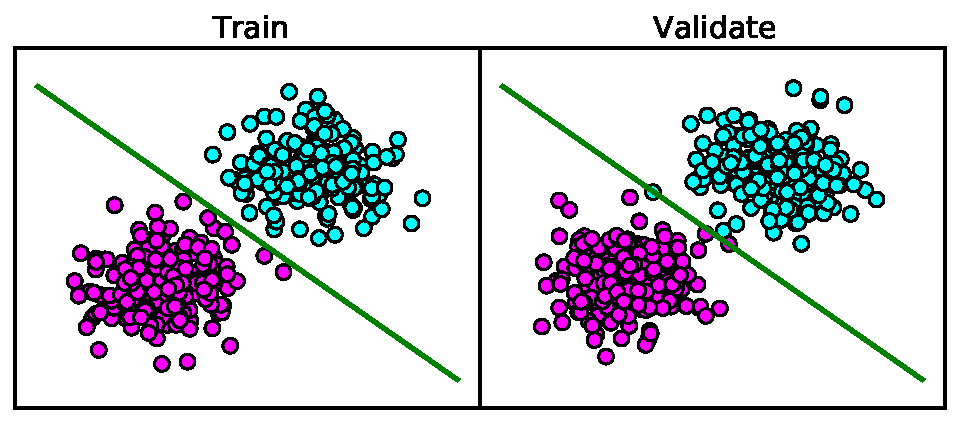
\includegraphics[width=.8\textwidth]{1-3-stdev1-1-0_15.pdf}
% 	\caption{stdev1}
% 	\label{fig:1-2-smalloverlap}
% \end{subfigure}
% \begin{subfigure}[b]{0.46\textwidth}
% 	\centering
% 	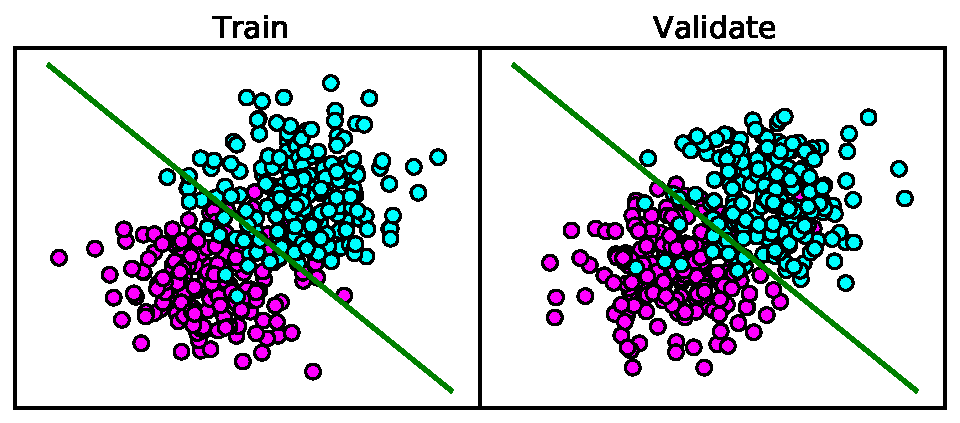
\includegraphics[width=.8\textwidth]{1-3-stdev2-10-0_15.pdf}
% 	\caption{stdev2}
% 	\label{fig:1-2-bigoverlap}
% \end{subfigure}
% \\
% \begin{subfigure}[b]{0.46\textwidth}
% 	\centering
% 	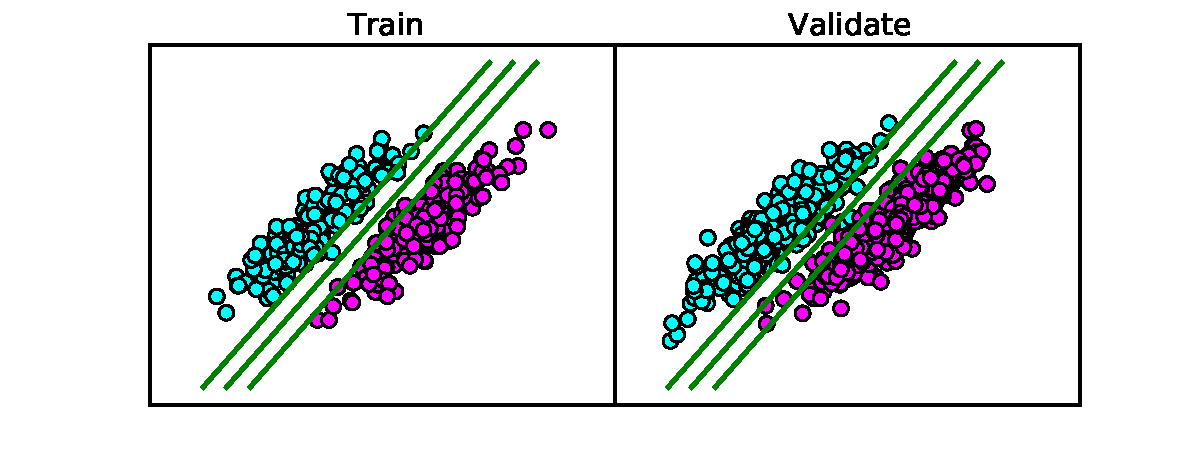
\includegraphics[width=\textwidth]{1-2-ls.pdf}
% 	\caption{ls}
% 	\label{fig:1-2-ls}
% \end{subfigure}
% \begin{subfigure}[b]{0.46\textwidth}
% 	\centering
% 	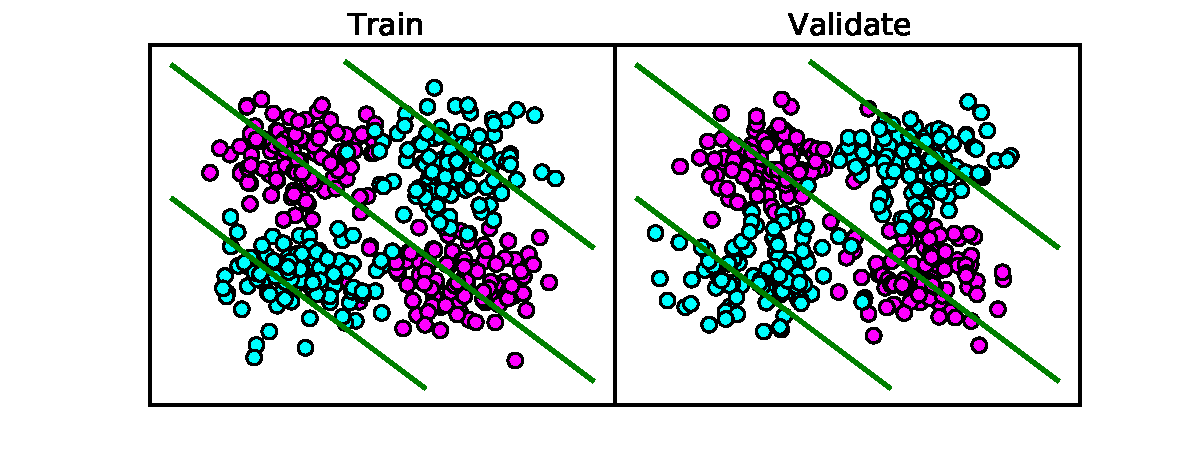
\includegraphics[width=\textwidth]{1-2-nonSep2.pdf}
% 	\caption{nonSep2}
% 	\label{fig:1-2-nonSep2}
% \end{subfigure}
% \end{figure}

Setting $C = 1$, the error rates for the training and validation sets for different data sets and kernels is shown in Table \ref{tbl:1-2-error}. If a data set did not come with a training / validation set pair, the dataset was randomly cut in half for each class to use as training and validation. In general, the more separable the data set is, the better the slack-variable SVM without a regularizer does. In the non-separable case, depending on the nature of the inseparability, the solution has a higher error rate.

\begin{figure}[!ht]
\centering
\begin{subfigure}[b]{0.46\textwidth}
	\centering
	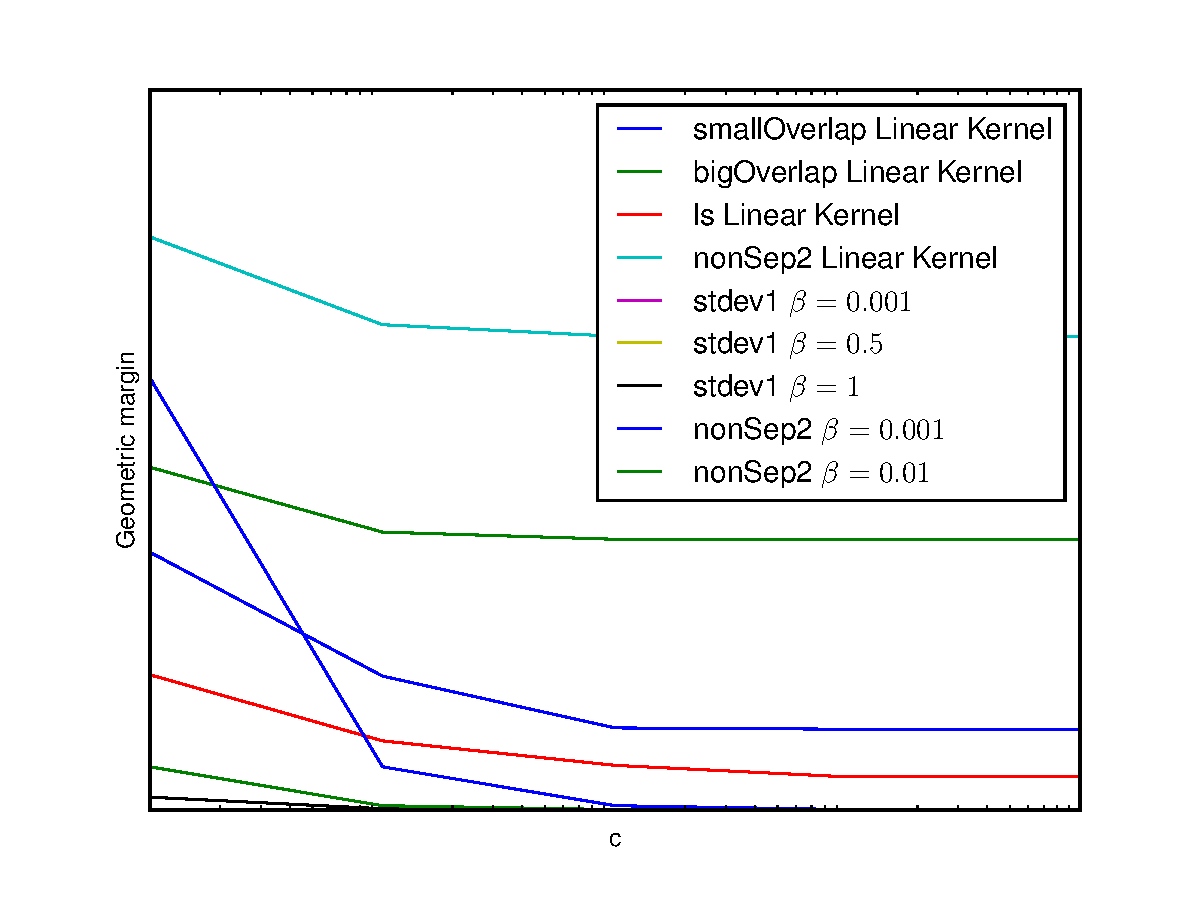
\includegraphics[width=\textwidth]{1-3-c-margin.pdf}
	\caption{plot of the geometric margin as a function of $c$ for various kernels and datasets}
	\label{fig:1-3-c-margin}
\end{subfigure}
\begin{subfigure}[b]{0.46\textwidth}
	\centering
	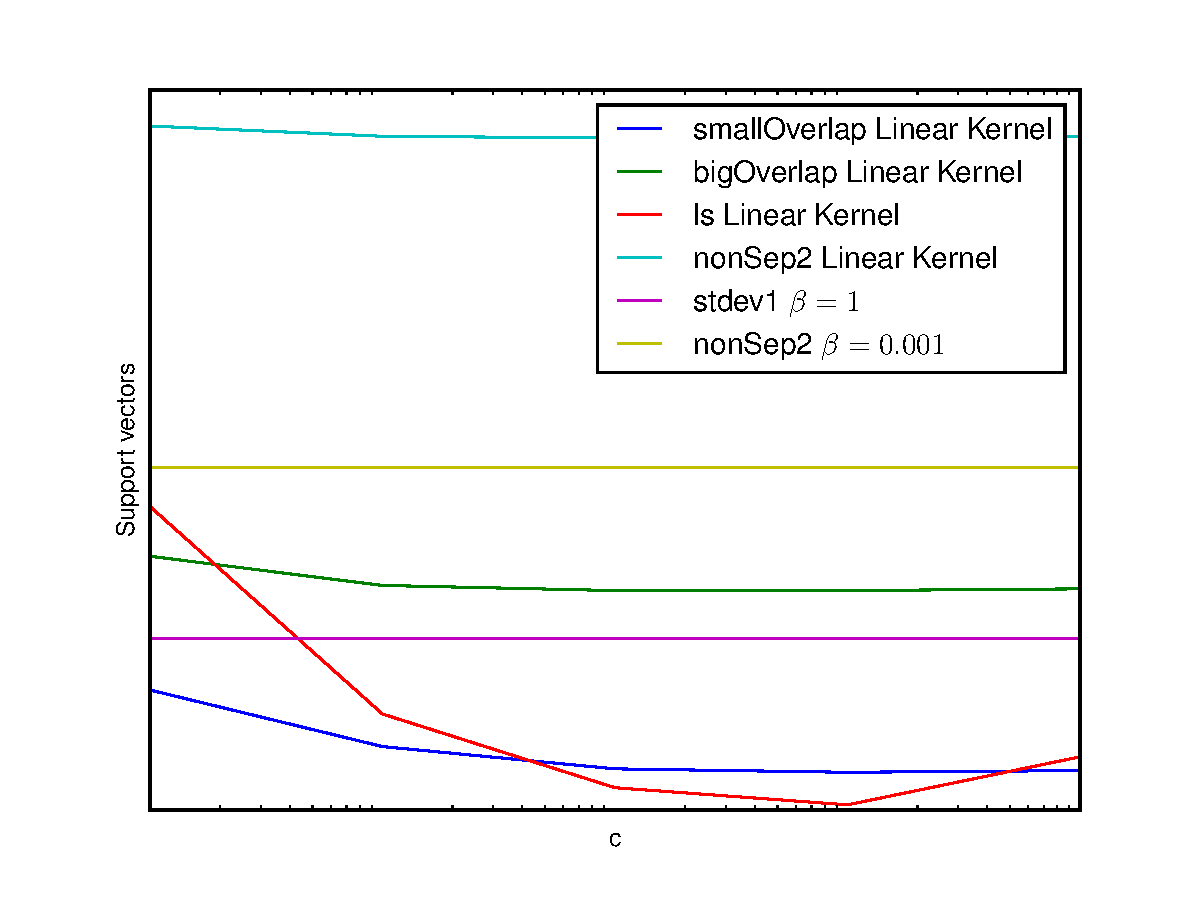
\includegraphics[width=\textwidth]{1-3-support-vectors.pdf}
	\caption{plot of the number of support vectors as a function of $c$ for various kernels and datasets}
	\label{fig:1-3-support-vectors}
\end{subfigure}
\caption{}
\label{fig:1-3-all}
\end{figure}

Extending the original Equation \ref{eq:singlesvm} to use kernels, the objective function becomes as written in Equation \ref{eq:singlesvmkernels} with corresponding prediction and $w_0$ calculation shown in Equation \ref{eq:singlesvm-predictor-kernels}. Using the Gaussian kernel compared to the linear kernel is shown in Figures \ref{fig:1-3-1}, \ref{fig:1-3-2}, \ref{fig:1-3-3}, and \ref{fig:1-3-4} for two different non-separable datasets. The Gaussian kernel allows for more flexibility in the classifier choosing non-linear segments that better-separate non-separable data. 

\begin{subequations}
\begin{align}
	S & \text{ is the set of support vectors (where )} \alpha > 0 \\
	y(x^{(t)}) &= \text{sign}\left(\sum_{i \in S}^n \alpha_i y^{(i)} K(x^{(t)}, x^{(i)}) + w0 \right)\\
	w_0 &= \frac{1}{|S|} \sum_{j \in S} \left(y^{(j)} - \sum_{i \in S} \alpha_i y^{(i)} K(x^{(i)}, x^{(j)}) \right)
\end{align}
\label{eq:singlesvm-predictor-kernels}
\end{subequations}

As you increase the bandwidth on a Gaussian kernel, the effect is that the separator for separable data gets more `rounded', while for non-separable data, the separator tends to find `pockets' of data that are moved into the separator for that class. Some results are shown in Figures \ref{fig:1-3-gaussian-small-beta}, \ref{fig:1-3-gaussian-larger-beta}, \ref{fig:1-3-gaussian-small-beta2}, and \ref{fig:1-3-gaussian-larger-beta2}. Both are tested on the same dataset (nonSep2) with the same value for $C$ ($C = 1$). For non-separable data, the performance is improved with increasing the bandwidth. Interestingly, when $\beta$ gets too small, the resulting decision boundary looks more linear (and has similar error rates to using a linear kernel for that value of $C$). For example, Figures \ref{fig:1-3-linear-linear} and \ref{fig:1-3-gaussian-linear} show a Gaussian kernel with small value of $\beta = 0.001$ and a linear kernel on the same dataset (stdev2) with $C = 1$ in both cases. The corresponding error rates are $.18$ for training and validation in both cases. 
Using a Gaussian kernel at different bandwidths does not change the error rates much unless the data is strongly non-separable, as shown in Table \ref{tbl:1-2-error}.

\begin{subequations}
\begin{align}
	\underset{\alpha}{\text{minimize}}
		& \quad -\sum_{i = 1}^n \alpha_i + \frac{1}{2} \sum_{i = 1}^n \sum_{j = 1}^n \alpha_i \alpha_j y^{(i)} y^{(j)} K(x^{(i)}, x^{(j)})) \\
	\text{subject to}
		& \quad 0 \leq \alpha_i \leq C \quad \forall i \,, \\
		& \quad \sum_{i = 1}^n \alpha_i y^{(i)} = 0
\end{align}
\label{eq:singlesvmkernels}
\end{subequations}

\begin{figure}[!ht]
\centering
\begin{subfigure}[t]{0.46\textwidth}
	\centering
	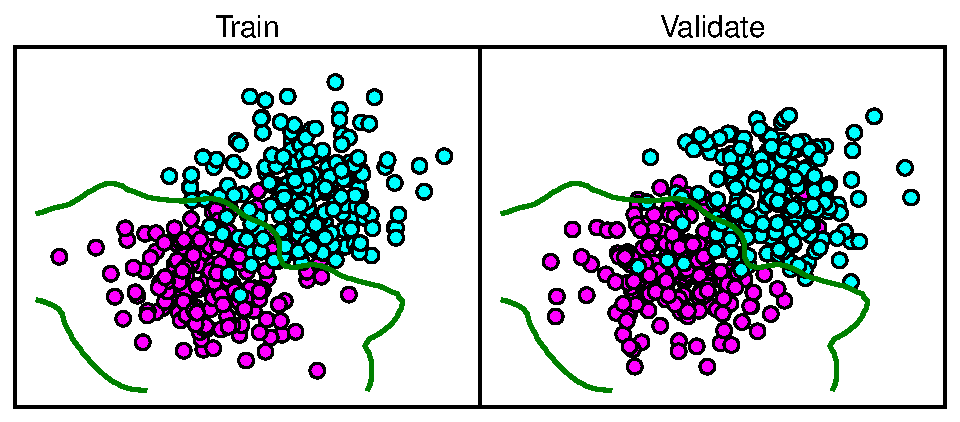
\includegraphics[width=.8\textwidth]{1-3-stdev2-0_1-1-gaussian-REAL.pdf}
	\caption{stdev2 using a Gaussian Kernel, $C = 0.1$, $\beta = 1$, Error = $.08$}
	\label{fig:1-3-1}
\end{subfigure}
\begin{subfigure}[t]{0.46\textwidth}
	\centering
	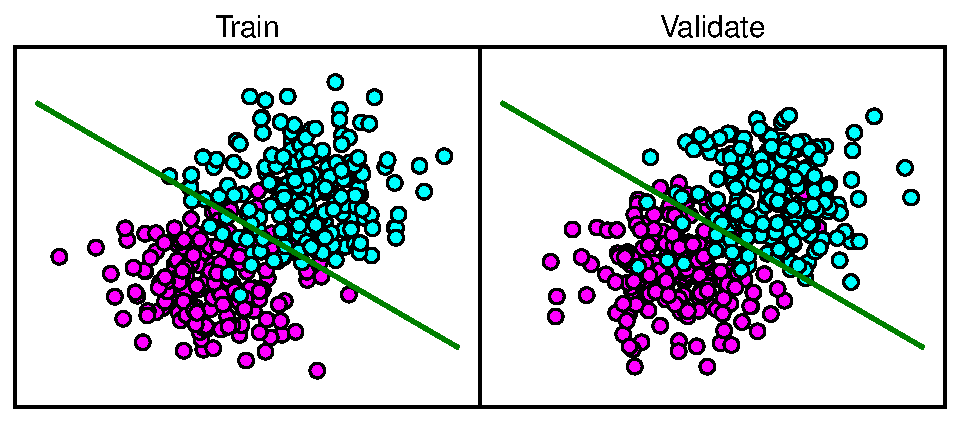
\includegraphics[width=.8\textwidth]{1-3-stdev2-0_1-linear-REAL.pdf}
	\caption{stdev2 using a Linear Kernel, $c = 0.1$, Error = $.20$}
	\label{fig:1-3-2}
\end{subfigure}
\\
\begin{subfigure}[t]{0.46\textwidth}
	\centering
	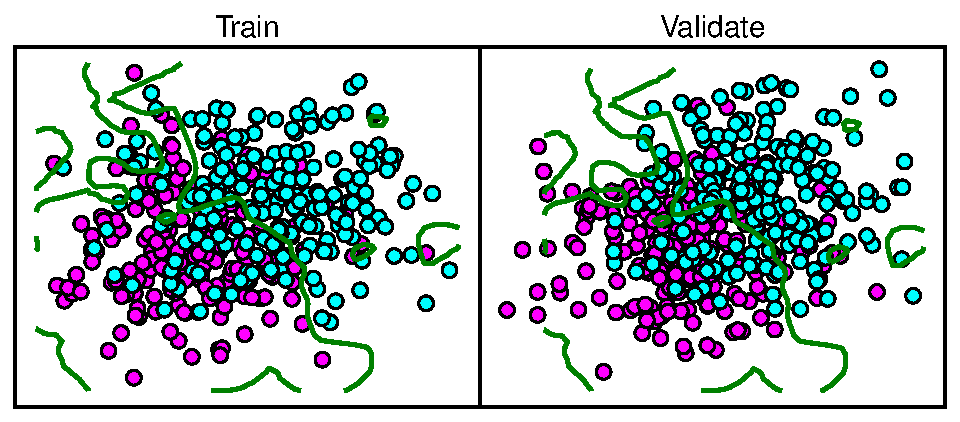
\includegraphics[width=.8\textwidth]{1-3-stdev4-0_01-1-gaussian-REAL.pdf}
	\caption{stdev4 using a Gaussian Kernel with $\beta = 1$, $C = 0.01$, Error = $.22$}
	\label{fig:1-3-3}
\end{subfigure}
\begin{subfigure}[t]{0.46\textwidth}
	\centering
	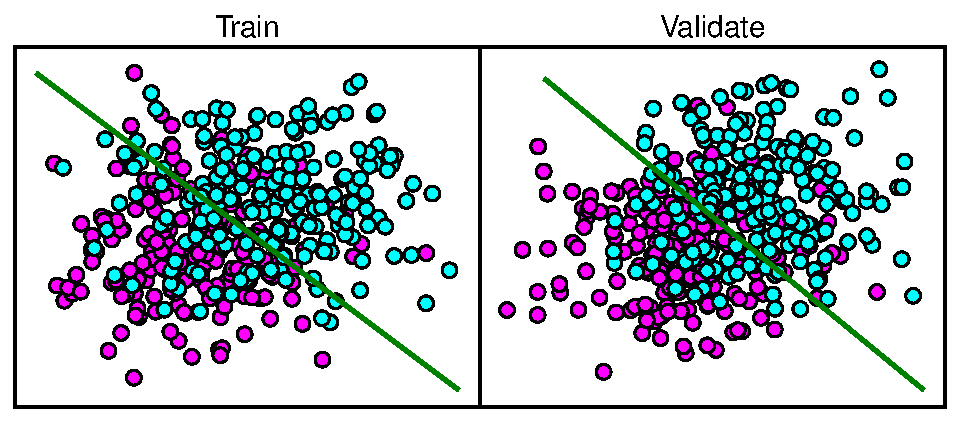
\includegraphics[width=.8\textwidth]{1-3-stdev4-0_01-linear-REAL.pdf}
	\caption{stdev4 using a Linear Kernel, $c = 0.1$, Error = $.45$}
	\label{fig:1-3-4}
\end{subfigure}
\caption{}
\label{fig:1-3-all2}
\end{figure}

\begin{figure}[!ht]
\begin{subfigure}[t]{0.46\textwidth}
	\centering
	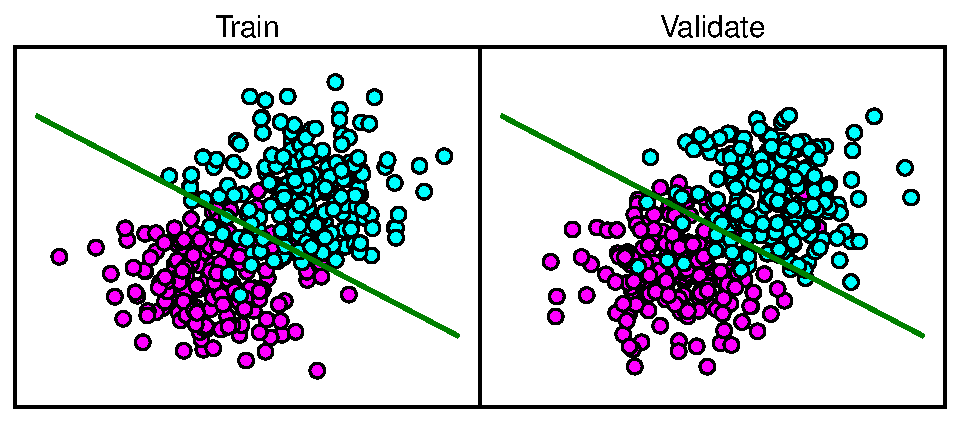
\includegraphics[width=.8\textwidth]{1-3-stdev2-1-linear-REAL.pdf}
	\caption{Linear kernel SVM on stdev2, $C = 1$. Error of $.18$.}
	\label{fig:1-3-linear-linear}
\end{subfigure}
\begin{subfigure}[t]{0.46\textwidth}
	\centering
	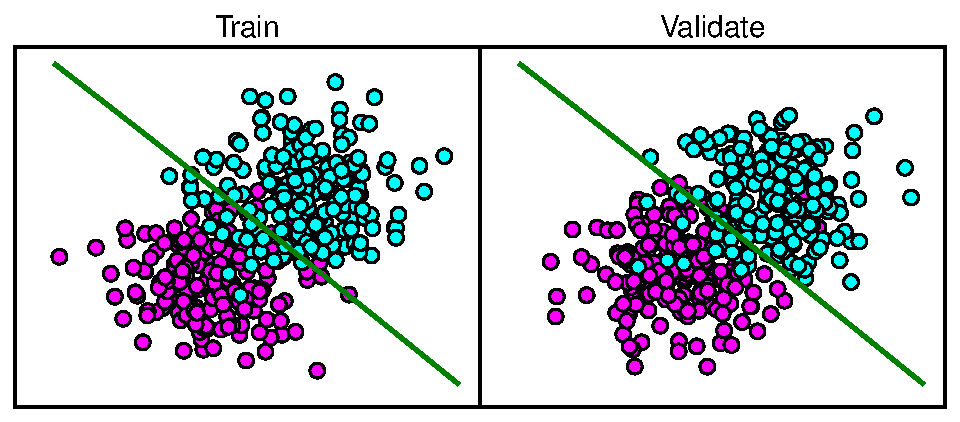
\includegraphics[width=.8\textwidth]{1-3-stdev2-1-0_001-gaussian-REAL.pdf}
	\caption{Gaussian kernel SVM with $\beta = 0.001$ and $C = 1$ on stdev2. Error of $.18$.}
	\label{fig:1-3-gaussian-linear}
\end{subfigure}
\caption{}
\label{fig:1-3-all3}
\end{figure}

As $c$ increases, the geometric margin decreases, as shown for various values of $c$, various kernels, and various datasets in figure \ref{fig:1-3-c-margin}. this always happens as $c$ increases, because this means there can be more slack in the final SVM, which means the SVM will be more tolerable to incorrect classifications for inseparable data. the number of support vectors first decreases, then increases as $c$ increases, as shown in figure \ref{fig:1-3-support-vectors}. this means that the classifier is less overfit on the training data and will have smaller errors on the testing data. choosing $c$ for maximizing the margin will yield a value of $c$ equal to zero, which is the same as having a hard-margin SVM that does not perform well on non-separable data. an alternate criteria for choosing $c$ could be the minimum number of support vectors (since the number of support vectors eventually increases with a higher value of $c$ as the classifier gets over-fit to the training data). Changing $c$ has almost no effect on the training error unless the data is highly non-separable.

\begin{figure}[!ht]
\begin{subfigure}[t]{0.46\textwidth}
	\centering
	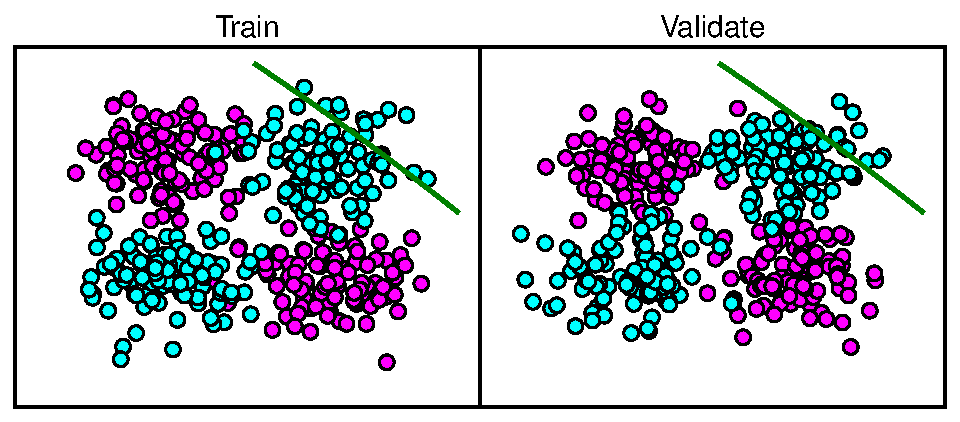
\includegraphics[width=.8\textwidth]{1-3-nonSep2-1-0_0001-gaussian-REAL.pdf}
	\caption{Gaussian kernel SVM on nonSep2, $C = 1$, $\beta = 0.0001$. Error of $.5$.}
	\label{fig:1-3-gaussian-small-beta}
\end{subfigure}
\begin{subfigure}[t]{0.46\textwidth}
	\centering
	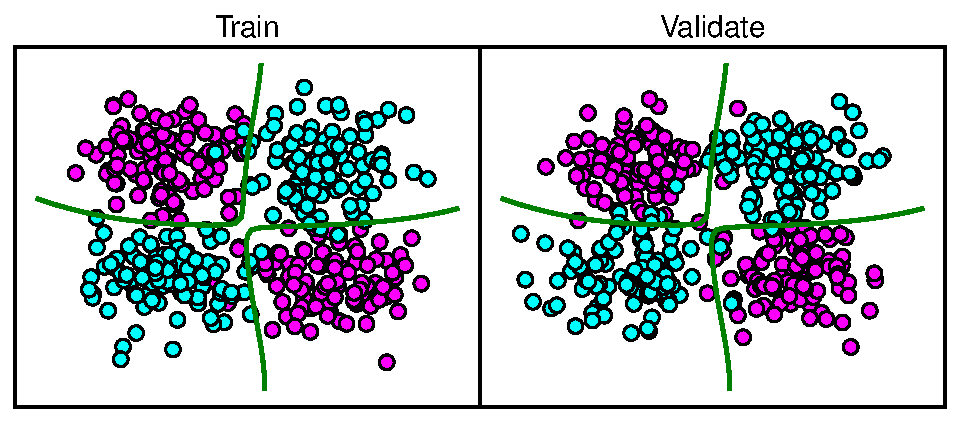
\includegraphics[width=.8\textwidth]{1-3-nonSep2-1-0_1-gaussian-REAL.pdf}
	\caption{Gaussian kernel SVM on nonSep2, $C = 1$, $\beta = 0.1$. Error of $.04$.}
	\label{fig:1-3-gaussian-larger-beta}
\end{subfigure}
\\
\begin{subfigure}[t]{0.46\textwidth}
	\centering
	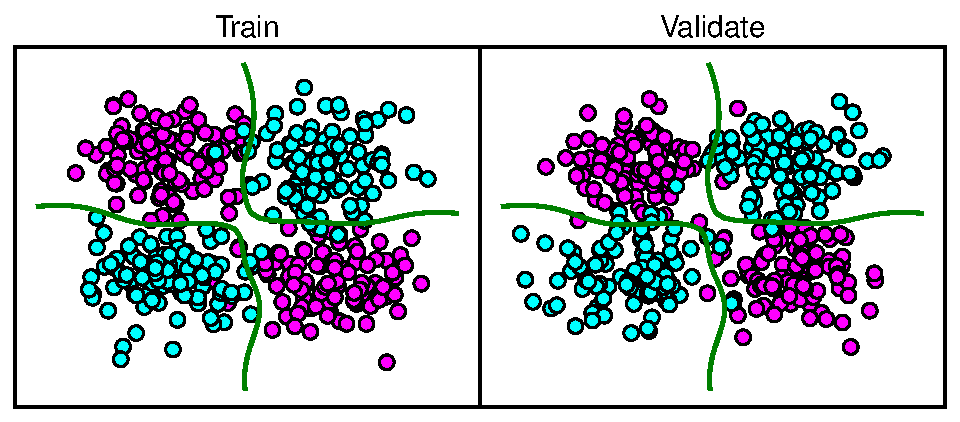
\includegraphics[width=.8\textwidth]{1-3-nonSep2-1-0_5-gaussian-REAL.pdf}
	\caption{Gaussian kernel SVM on nonSep2, $C = 1$, $\beta = 0.5$. Error of $.04$.}
	\label{fig:1-3-gaussian-small-beta2}
\end{subfigure}
\begin{subfigure}[t]{0.46\textwidth}
	\centering
	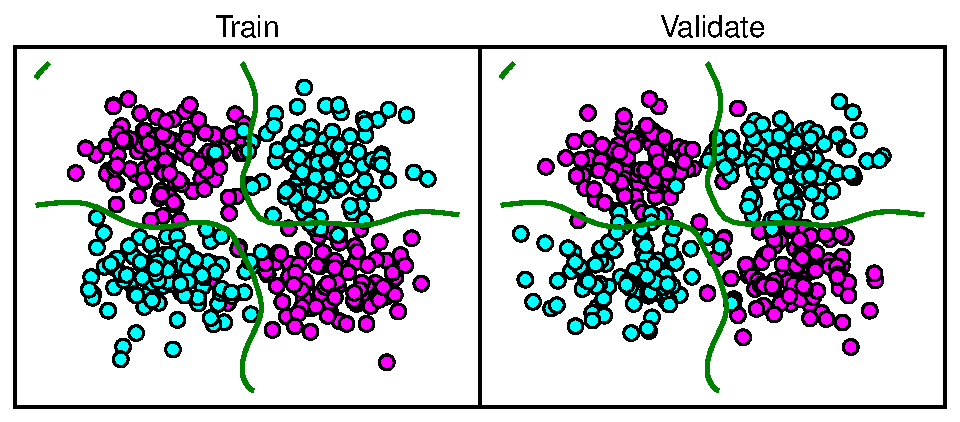
\includegraphics[width=.8\textwidth]{1-3-nonSep2-1-1-gaussian-REAL.pdf}
	\caption{Gaussian kernel SVM on nonSep2, $C = 1$, $\beta = 1$. Error of $.04$.}
	\label{fig:1-3-gaussian-larger-beta2}
\end{subfigure}
\caption{}
\label{fig:1-3-all4}
\end{figure}

\section{Exercise 2: Logistic Regression}

The kernelized form of the regression objective and the associated prediction function I used for logistic regression having all data with $y^{(i)} \in {-1, 1}$ is written in Equation \ref{eq:kernelized-lr}. $K$ is the kernel function, which in the linear case is $x^{(i')} \cdot x^{(i)}$. For accurate results, it was important to set the tolerance of the solver to $1e^{-12}$. The solver is then used to optimize over the values of $\alpha$ and $w_0$ at the same time.

\begin{subequations}
	\begin{align}
		\text{NLL}(\alpha, w_0) &= \sum_i \log \left(1 + e^{-y^{(i)}\left(\displaystyle\sum_{i'} \alpha_{i'} K(x^{(i')}, x^{(i)}) + w_0\right)}\right) \\
		y(x_t) &= \text{sgn}\left(w_0 + \sum_i \alpha_i K(x^{(i)}, x_t)\right)
	\end{align}
	\label{eq:kernelized-lr}
\end{subequations}


\begin{figure}[!ht]
\begin{subfigure}[t]{0.46\textwidth}
	\centering
	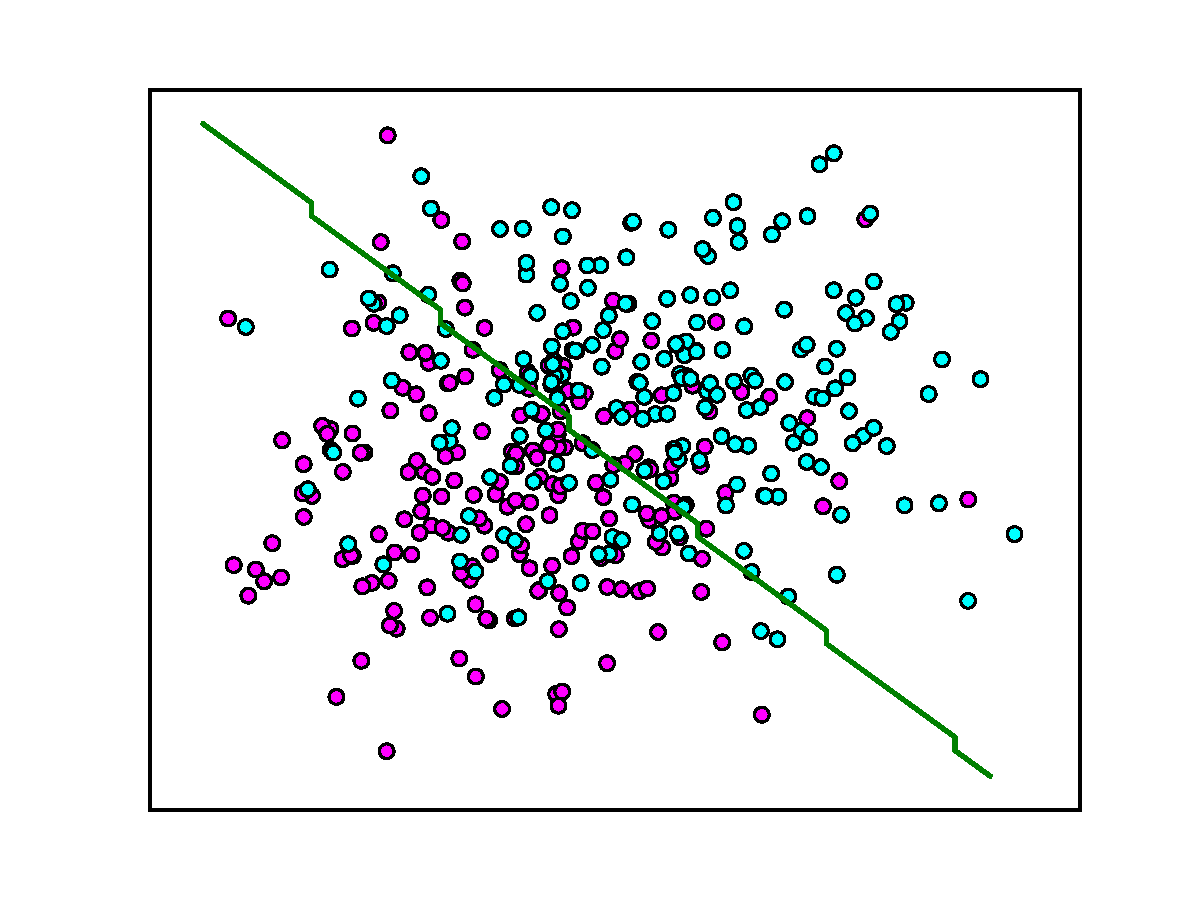
\includegraphics[width=\textwidth]{exercise2-3-stdev4-linear.pdf}
	\caption{Decision boundary on non-separable data for linear kernel. Error = $.265$}
	\label{fig:2-3-linear}
\end{subfigure}
\begin{subfigure}[t]{0.46\textwidth}
	\centering
	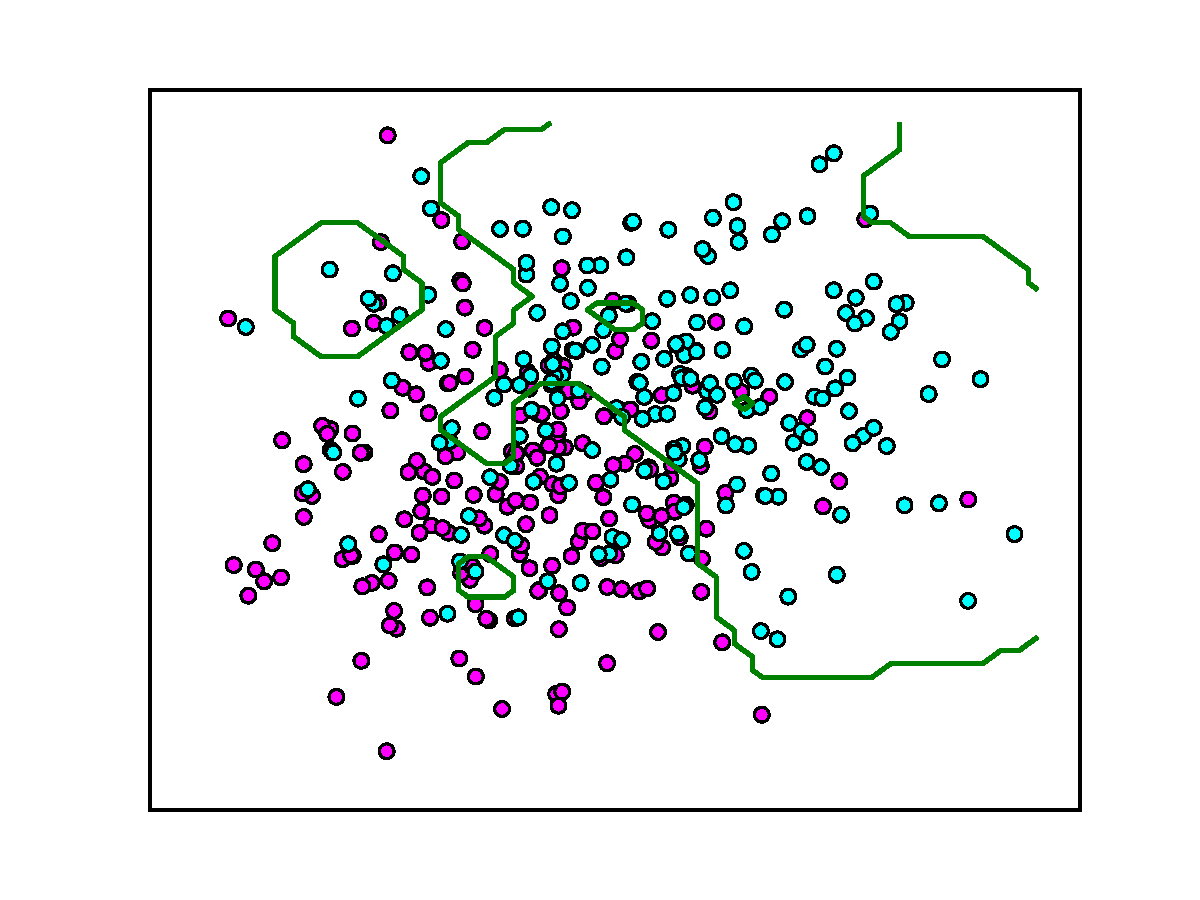
\includegraphics[width=\textwidth]{exercise2-3-stdev4-gaussian.pdf}
	\caption{Decision boundary on non-separable data for Gaussian kernel. Error = $.2625$}
	\label{fig:2-3-gaussian}
\end{subfigure}
\caption{}
\label{fig:2-3-all}
\end{figure}

When comparing Gaussian kernels and linear kernels on the same dataset, Gaussian kernels perform much better on non-separable datasets. The decision boundaries on the same dataset (stdev4, which is highly non-separable) using a linear and a Gaussian kernel (with $\beta = $ chosen using the minimum training set error while holding $\lambda = 0$) is shown in Figures \ref{fig:2-3-linear} and \ref{fig:2-3-gaussian}. In this case the optimal value of $\beta$ was $0.2$ The corresponding error rates on the test set are $.265$ for the linear kernel and $.2625$ for the Gaussian kernel. When computing the Gaussian kernel, the maximum number of iterations of the minimization function was set to reduce computation time.

\begin{figure}[!ht]
\begin{subfigure}[t]{0.46\textwidth}
	\centering
	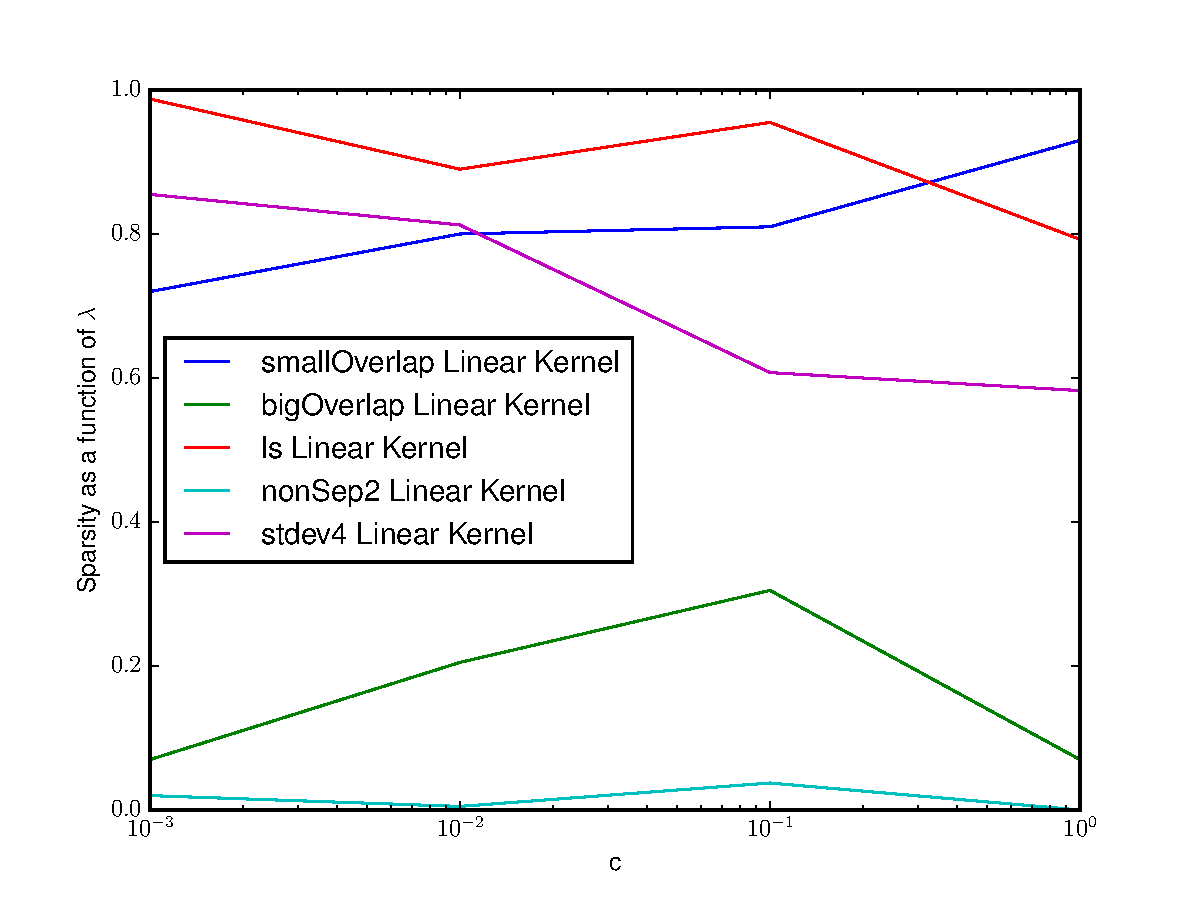
\includegraphics[width=\textwidth]{exercise2-2.pdf}
	\caption{Sparsity as a function of $\lambda$ for the linear kernel}
	\label{fig:2-2}
\end{subfigure}
\begin{subfigure}[t]{0.46\textwidth}
	\centering
	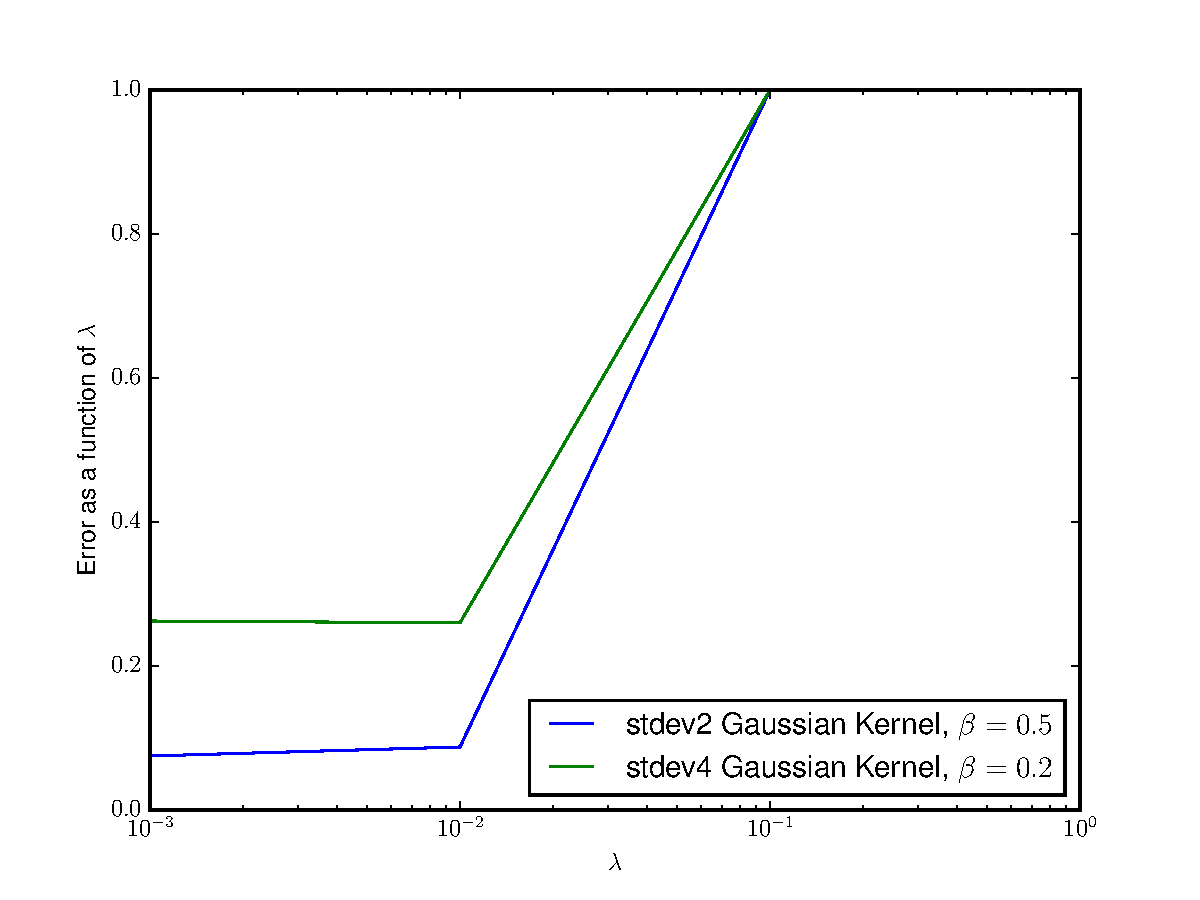
\includegraphics[width=\textwidth]{exercise2-4.pdf}
	\caption{Error as a function of $\lambda$ and $\beta$ for Gaussian kernels}
	\label{fig:2-4}
\end{subfigure}
\caption{}
\label{fig:2-2-2-4-all}
\end{figure}

Define sparsity as the percentage of points in the training data that are used as support vectors (with alpha values greater than $1e^{-5}$. Using L1 regularization with parameter $\lambda$ on the $\alpha$ values to ensure sparsity, the relationship between $\lambda$ and sparsity is shown in Figure \ref{fig:2-2} for various datasets for the linear kernel. In general, the sparsity follows a U-pattern, sometimes in two places, as $\lambda$ increases. The optimal value of $\lambda$ is the one that in the separable case makes the sparsity the lowest for the smallest value of $\lambda$. As $\lambda$ gets too large, the error on the training and testing sets increases too much, so it is better to choose a smaller value of $\lambda$ that allows for low training / testing error. In the non-separable case, the sparsity either follows a U-shape or decreases as $\lambda$ increases.

The performance of the Gaussian kernel depends on choosing the optimal $\beta$. In general, the optimal $\beta$ is the near the standard deviation of the distribution of the data. The effect of $\lambda$ on performance once the optimal $\beta$ is chosen is shown in Figure \ref{fig:2-4}. In general, the affect of $\lambda$ on the error is a U-shape, and the optimal $\lambda$ should be chosen to minimize the validation set error after the value of $\beta$ has already been chosen.

Comparing SVMs to logistic regression in terms of sparsity, logistic regression tends to be more sparse than SVM, and the support vectors chosen in SVM dictate the boundary more strongly.

\section{Exercise 3: Multiclass LR and SVM}

\subsection{Multiclass Logistic Regression}

The form of the objective for kernelized multiclass logistic regression is the same as for the two-class case shown in Equation \ref{eq:kernelized-lr}, except that the $y$ values are $1 \times K$ vectors where $K$ is the total number of classes. All the entries in $y$ are $0$ except for the entry that corresponds to the class that $y$ belongs to, which is $1$. So if $x^{(i)}$ were in class $3$ out of a total of $5$ classes, $y^{(i)}$ would take on the value $[0, 0, 1, 0, 0]$. The resulting prediction function was then modified as shown in Equation \ref{eq:multiclass-lr}. So for each class $c$ there is a separate set of $\alpha$ and $w_0$ values, and the class that is predicted is the class who's $\alpha$ and $w_0$ values maximize the objective function. 

When the solver is run, the tolerance is set to $1e^{-12}$ to both get numerically salient results and to try to avoid overflow errors in the solver. The solver optimizes over all the values of $\alpha$ and $w_0$ for all classes simultaneously, causing the solver to take a long time to process all the matrix multiplications. If there are $c$ classes and $n$ training points, there are $c$ corresponding values for $w_0$ (one for each class), so there are a total of $c(n + 1)$ parameters being optimized over simultaneously.

\begin{subequations}
	\begin{align}
		y = \underset{c}{\text{argmax}} \left(w_{c0} + \sum_i \alpha^c_i K(x^{(i)}, x_t)\right)
	\end{align}
	\label{eq:multiclass-lr}
\end{subequations}

There were numerous problems in implementing logistic regression for multiclass, especially on running the Kaggle dataset. There were many features and many data points, so it was especially important not to have any operations involving for loops, doing everything with the optimized versions of Python's numpy / scipy library. Another trick I used was to use the $\text{logexpsum}$ function from the scipy library to calculate the error in the objective function as needed. At all places possible, I used built-in functions in scipy and numpy to do any calculations rather than write it by hand. For most experiments with logistic regression, the regularization term was L1 regularization to keep the $\alpha$ values sparse. It was also important to always initialize the starting value of the minimization function to zeros rather than using numpy's built-in `empty' function for creating arrays. This is because using the `empty' function reuses empty places in memory (most likely taken by the coefficients from the previous run of the minimization), therefore causing the function to be stuck in a local minimum.

Experimenting on small subsets of Kaggle data with linear and Gaussian kernels, it was immediately clear that with a Gaussian kernel and a relatively small number of data points (approximately $10$) and a Gaussian kernel, there can immediately be an error rate of $0.0$ on the validation set. Therefore, for all larger experiments, only the Gaussian kernel was used when doing multiclass logistic regression. The linear kernel assumes that the data are more separable than they really are, so the Gaussian kernel was used to exploit the possibility of decision boundaries being in infinite-dimensional spaces that are not necessarily separable.

In about 20-30 minutes of run time, I used all 54 features and 40 training samples from each class for a training and validation set, randomly selected without replacement. I used the training set to choose the optimal value of $\beta$ while holding $\lambda = 0$, then I used the validation set to choose the optimum value of $\lambda$, and finally tested on the rest of the un-chosen values of the dataset. After a few runs, the results were that the best $\beta$ value was $\beta = 2$ and the best $\lambda$ was $\lambda = 0.001$ for an error rate of $.83$ on the entire dataset.

Potential performance improvement to multiclass logistic regression are discussed in Section \ref{sec:improvement}.

\subsection{Multiclass SVM}

For multiclass SVM, it was also critical not to use any for loops or unnecessary mathematical operations. Using the one-versus-rest approach in which $K$ separate SVMs of the form written in Equation \ref{eq:singlesvm} are trained and optimized where the $k$th SVM is trained from class $C_k$ as positive examples and the rest of the classes as negative examples. The predictor is then of the form written in Equation \ref{eq:multiclassvm}. The important part here is that the sign of the predictor function is not relevant - the relevant part is the largest value that pops out of the predictor, since there are multiple options. This is why the `sign' function from the single-class case is removed, replaced with an `argmax' function for which value $k$ returns the maximum predicted value from one predictor.

\begin{subequations}
	\begin{align}
		y &= \underset{k}{\text{argmax }} y_k(x) \\
		y_k (x^{(t)}) &= \sum_{i \in S}^n \alpha_{ki} y^{(i)} K(x^{(t)}, x^{(i)}) + w_{0k} \\
		w_{0k} &= \frac{1}{|S|} \sum_{j \in S} \left(y^{(j)} - \sum_{i \in S} \alpha_{ki} y^{(i)} K(x^{(i)}, x^{(j)}) \right)
	\end{align}
	\label{eq:multiclassvm}
\end{subequations}

The QP solver just solves for the values of $\alpha$ for each class, so if there are $k$ classes and $n$ training samples, there are $k$ predictors created, each with $n$ parameters. The values of $w_0$ for each class are calculated after the predictors are computed by the solver. 

When splitting the data into three sets: train, validation, and test, it was important to randomly select the indices used for training, validation, and test in case the data were sorted in some way. 

From a few small tests on the Kaggle data, it was immediately obvious that a Gaussian kernel was more suited to the problem rather than a linear kernel. Even for small numbers of training points (around $20$), with a linear kernel and a large value of $C$, the errors were in the $.3$ range for training. For similarly-sized datasets and the Gaussian kernel, the training errors were already tending towards $0$. For all the larger tests I did, I used a Gaussian kernel and selected a value for $\beta$. In many cases for small data sets, the data was separable for all values of $\beta$ so the training error was zero. The validation set was used to select for the optimal combination of $c$ and $\beta$.

In my implementation, In about 30 minutes of computation time for training, validation, and testing using a Gaussian kernel, I was able to use about $1000$ data points and all the features for training and validation. To find the optimal values of $\beta$ and $c$, they were pairwise tried on all the data points, first selecting for the optimal value of $\beta$, then the value of $c$. The optimal value of $\beta$ was found to be $1$ and the optimal value of $c$ was usually $0.1$. The training error was often $0$, and the validation and training errors were hovering around $.3$. In my best run, the test error on the entire dataset was $.4$. 

To test my implementation against a professional implementation in an attempt to use all the data points for training, the `sklearn' Python package was used to perform SVM on the entire Kaggle Forest dataset. One major drawback of using this package the super-fast package did not implement Gaussian kernels, so the results given here are using linear kernels. Using hinge loss and L2 regularization, the optimal value for $\lambda$ was $0.01$ and the test error was $.261$ on the entire dataset. Using squared loss and L1 regularization, the optimal $\lambda$ was $1e^{-7}$ and the test error was $.143$. Unfortunately, this implementation did not test using Gaussian kernels. With a longer computation time on my implementation using Gaussian kernels, I think the error rates will be smaller using a Gaussian kernel.

Potential performance improvement to multiclass SVM are discussed in Section \ref{sec:improvement}.

\subsection{Multiclass SVM and Logistic Regression Areas of Improvement}
\label{sec:improvement}

A big blocker in multiclass logistic regression is the computation required for the gradient descent function. The problem with the multiclass problem rather than the single class logistic regression problem is the number of variables to simultaneously optimize. With each added class, the multiclass version grows with the number of training samples (especially in the kernelized version). So to make multiclass logistic regression faster, either a better gradient descent solver or a larger memory cache is necessary, so that all of the variables to be optimized can be kept in memory at the same time.

One huge area of improvement for multiclass SVM is to find a QP solver that evaluates faster results using a $C$ implementation of quadratic programming. Another potential improvement is to reduce the feature space on the Kaggle training set (relevant for both multiclass logistic regression and multiclass SVMs), so that only the features that prove the most predictive are considered in the training algorithms. This can be accomplished by training on a small number of data points with a subset of features in a one-vs-rest classifier scheme for SVM, seeing which subset of features produces the most effective results on a small set of data.

Another improvement I explored was using native Python implementations of Gaussian (RBF) kernels. The `sklearn' Python kit provides a native implementation of Gaussian kernels that performs faster than my implementation.

\end{document}